\chapter{Appendix}
\label{sec:appendix}

\section{Paper I}
\vfil\null
\huge{\textbf{Influence of Meteorological Conditions on Artificial Ice Reservoir (Icestupa) Evolution}}

\bigskip
\large{Balasubramanian, S., Hoelzle, M., Lehning, M., Bolibar, J., Wangchuk, S.,
  Oerlemans, J., and Keller, F. \par  Frontiers in Earth Science 9 (February 23, 2022): 771342.\par
doi:10.3389/feart.2021.771342.}

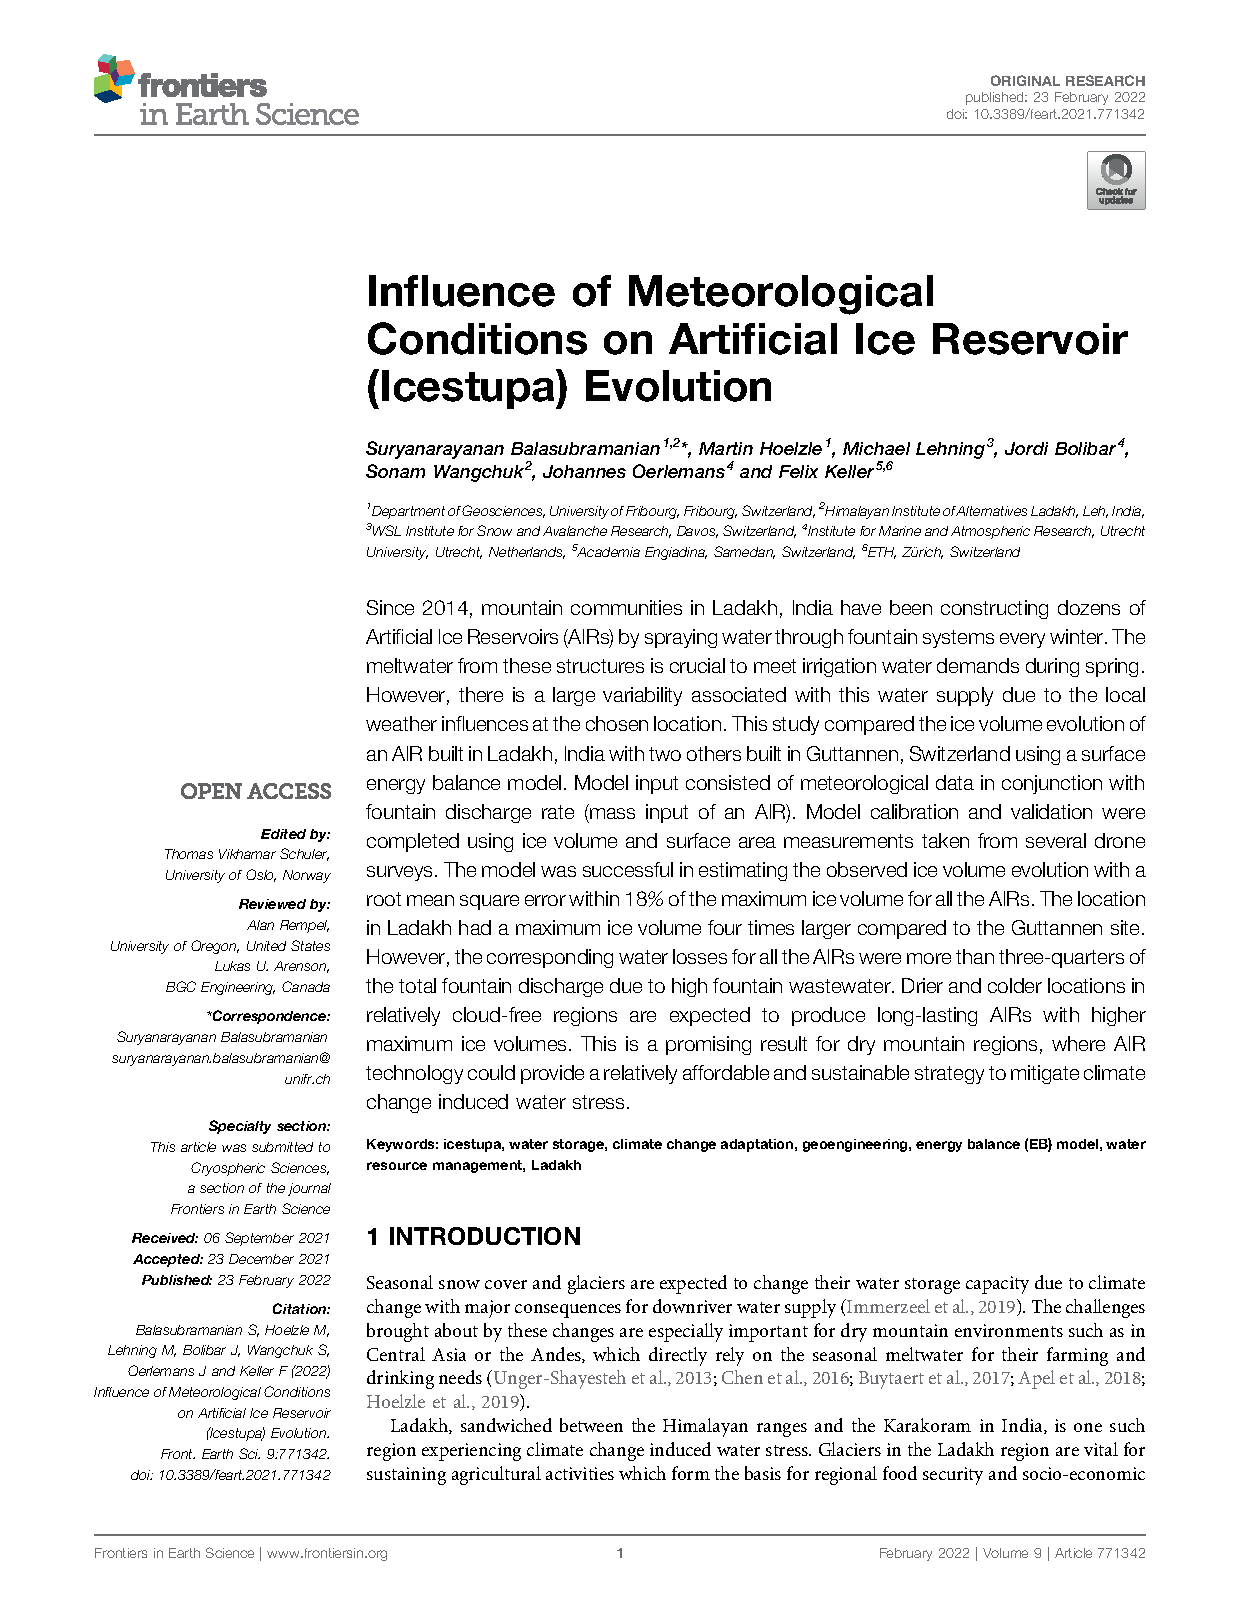
\includepdf[pages=-,pagecommand={},width=\paperwidth, scale=10]{content/papers/paperI.pdf}

\section{Paper II}
\vfil\null
\huge{\textbf{Fountain scheduling strategies for improving water-use efficiency of artificial ice reservoirs (Ice stupas)}}

\bigskip
\large{Balasubramanian, S., Hoelzle, M., and Waser, R. \par  Cold Regions Science and Technology (October 30,
2022) \par doi:10.1016/j.coldregions.2022.103706 }

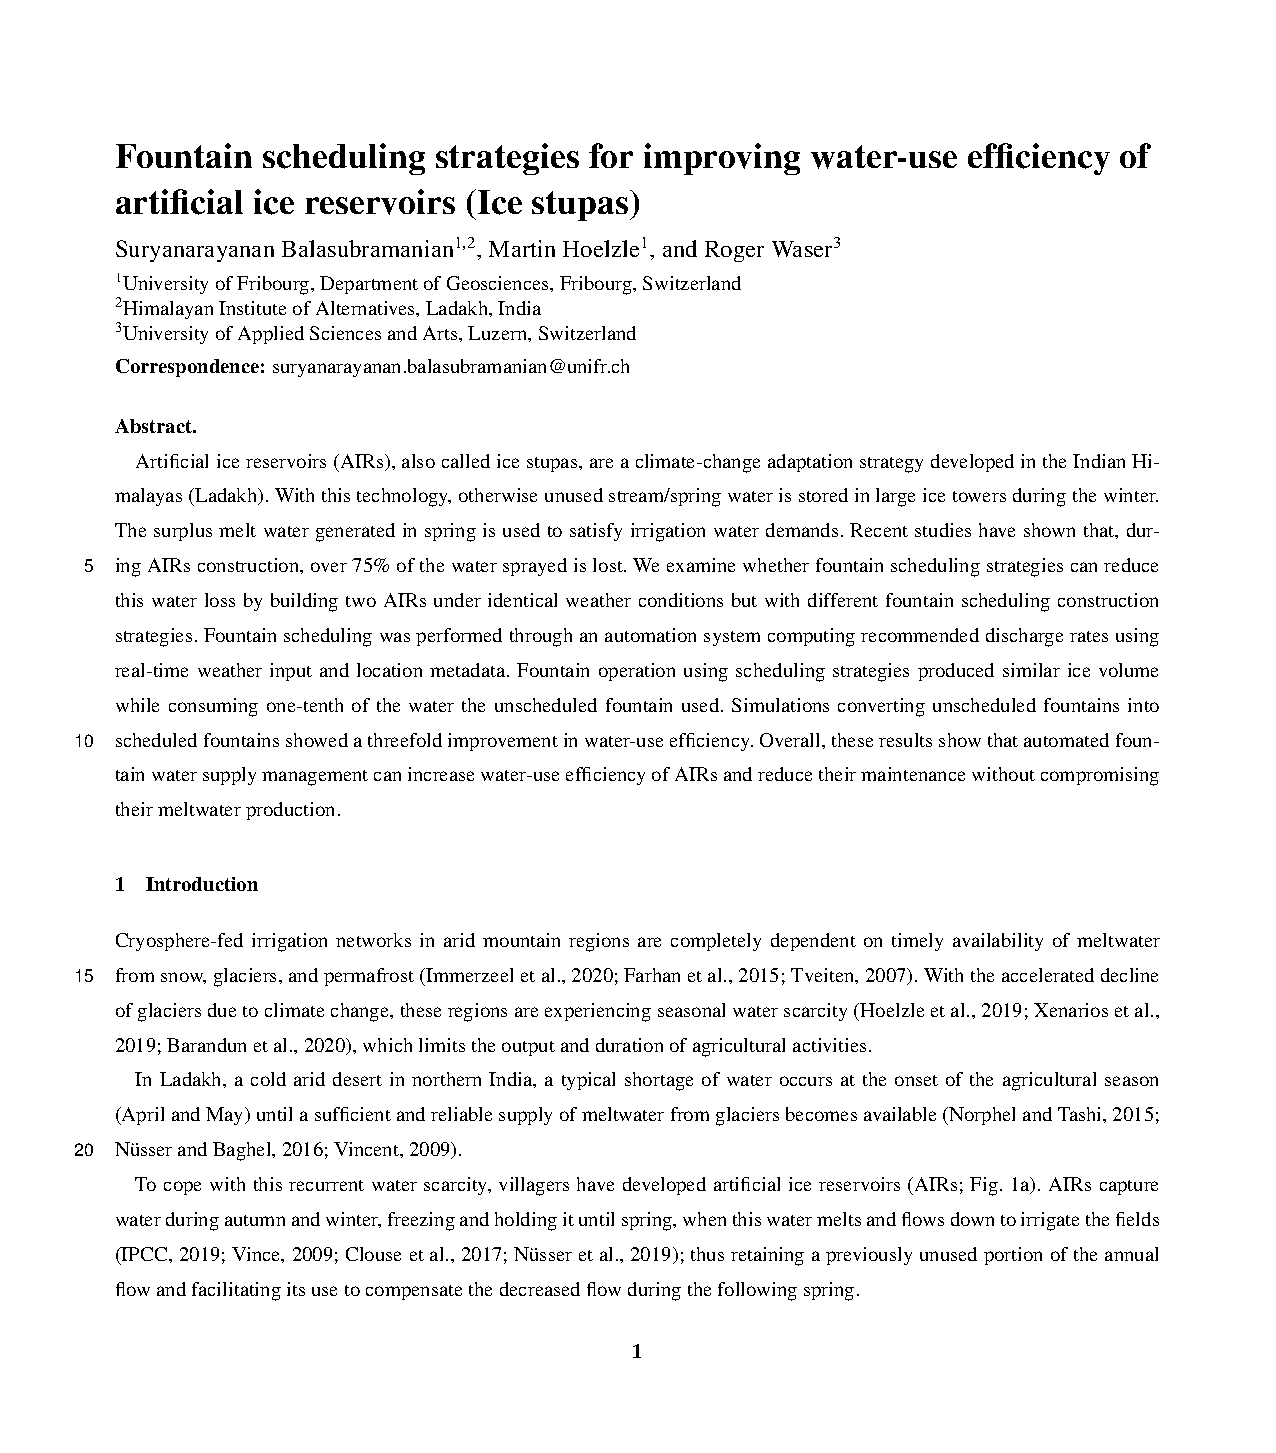
\includepdf[pages=-,pagecommand={},width=\paperwidth, scale=10]{content/papers/paperII.pdf}

% \section{Co-authored papers}
\section{Paper III}
\vfil\null
\huge{\textbf{Brief communication: Growth and decay of an ice stupa in alpine conditions – a simple model driven by energy-flux observations over a glacier surface}}

\bigskip
\large{
Oerlemans, J., S. Balasubramanian, C. Clavuot, and F. Keller. \par The Cryosphere 15, no. 6 (2021): 3007–12.
\par doi:10.5194/tc-15-3007-2021.
  }

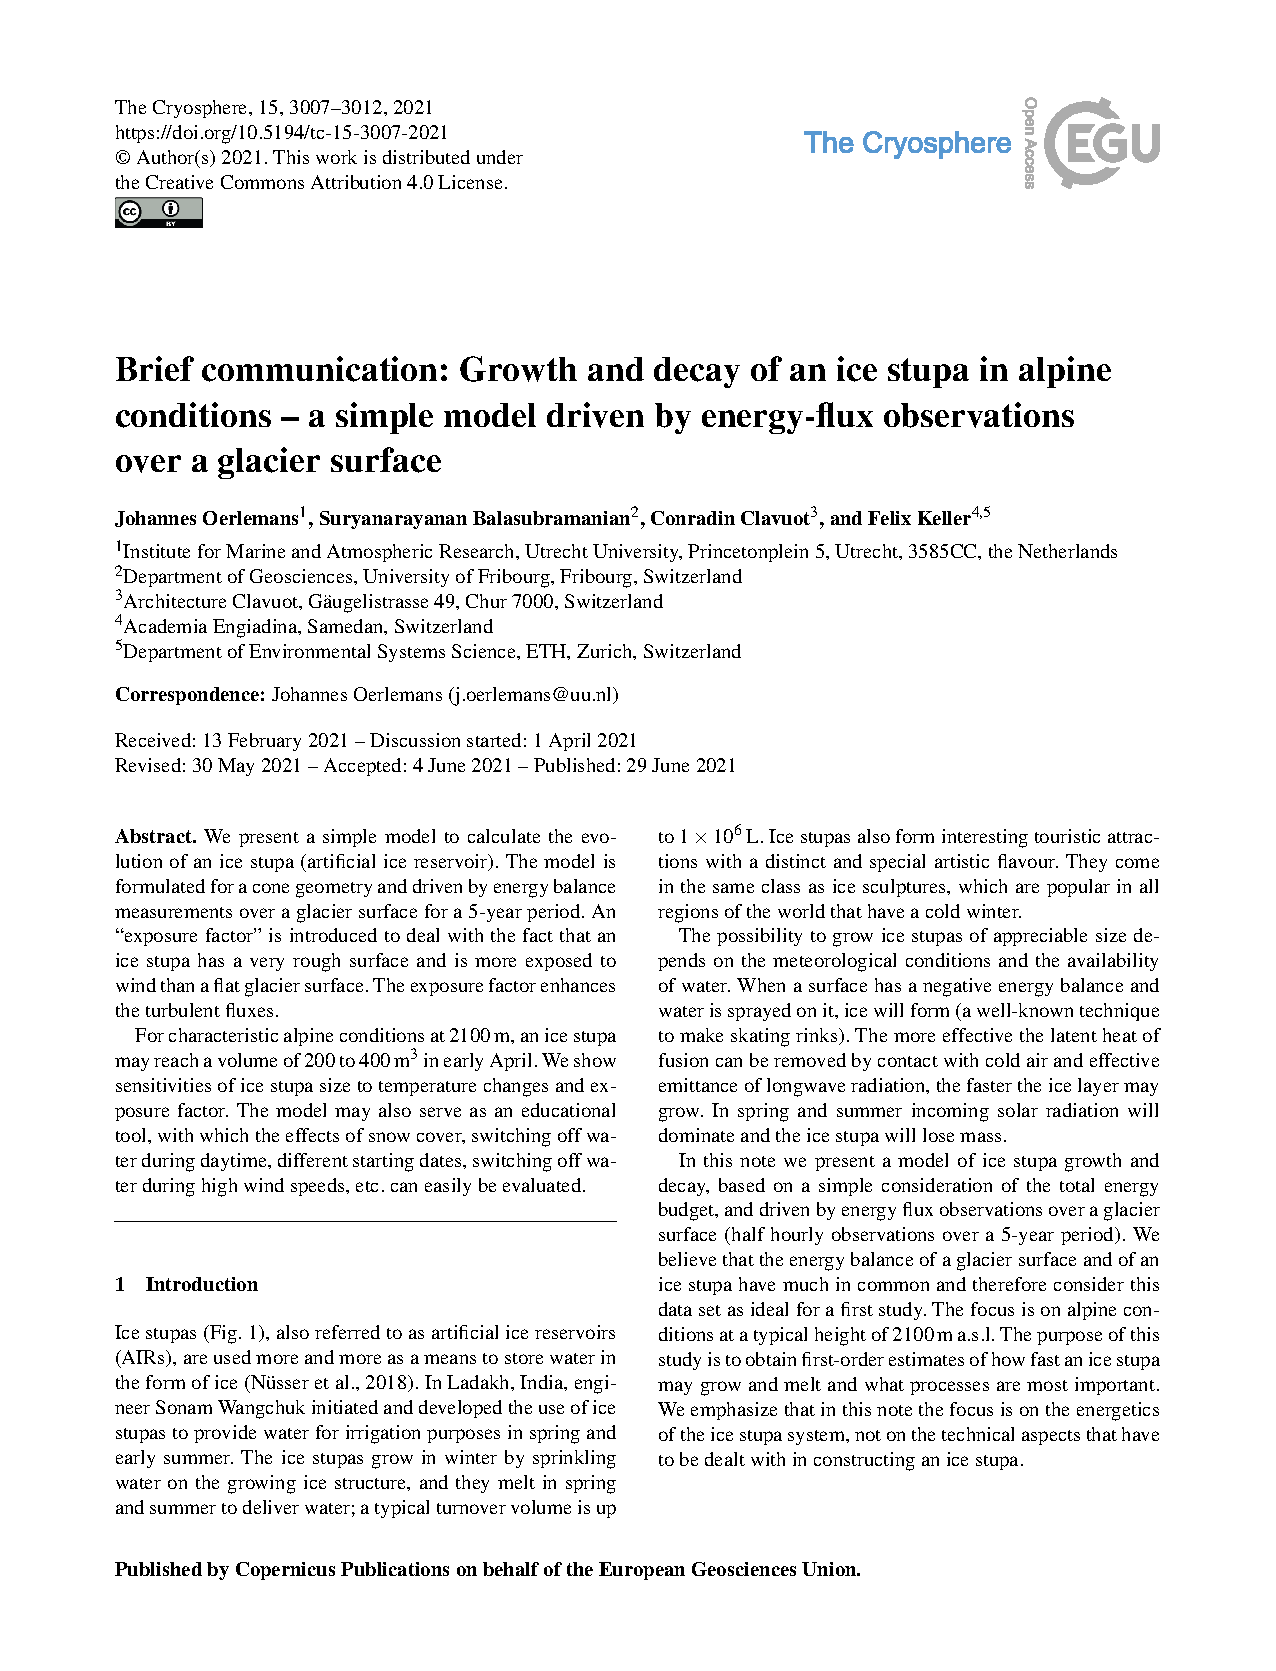
\includepdf[pages=-,pagecommand={},width=\paperwidth, scale=10]{content/papers/paperIII.pdf}

\section{Drone surveys and their processing methodology}
\label{sec:drone_method}

The drone flew along a predefined flight course and took photographs at set time intervals. The
position and altitude of the drone at the exposure stations, which were obtained by the built-in integrated
position and orientation system (POS, composed of a global positioning system and inertial measurement units),
were recorded in JPEG pictures. In the present work, we adopted a three-step workflow, as implemented in the
commercial software package Pix4Dmapper version 4.6.4 (\cite{pix4dsaPix4DmapperUserManual2020}). A short summary of this workflow is
described below:

\begin{figure}
	\begin{center}
		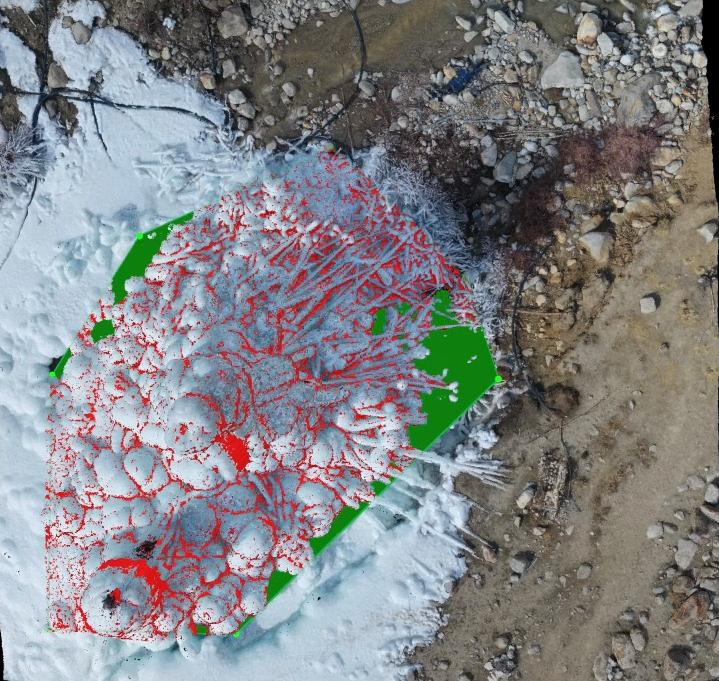
\includegraphics[width=12 cm]{figs/pix4d.jpg}
	\end{center}
	\caption{Digital elevation map of Indian \ac{AIR} constructed from the drone survey on March 3, 2021. The green
		area represents the area bounded by the marked perimeter, and the red area represents gaps in the point cloud
    that were filled to compute the associated volume.
	}
	\label{fig:DEM}
\end{figure}

(1) Initial processing: This process generates a sparse point cloud with the structure-from-motion algorithm
(\cite{turnerAutomatedTechniqueGenerating2012}). First, it searches for and matches key points in the photos which present certain overlapping
areas using a feature matching algorithm (e.g., the scale-invariant feature transform (SIFT) algorithm, which can
detect key points in photos under different views and illumination conditions;
\cite{loweDistinctiveImageFeatures2004}). Second, the approximate locations and orientations of the camera at
each exposure station are reconstructed with the internal parameters (focal length, coordinates of the principal
point of the photograph) and external parameters (i.e., POS data). A sparse point cloud is created.

(2) Point cloud densification: In this step, the multiview stereo technique is applied to achieve a higher
point cloud density than that in the previous step (\cite{furukawaAccurateDenseRobust2010};
\cite{molgStructurefromMotionUsingHistorical2017}). Thus, the spatial resolution of the products can be
increased, and an irregular network for the next step can be created (\cite{kungACCURACYAUTOMATICPHOTOGRAMMETRIC2011}).

(3) \ac{AIR} delineation: Ice radius, area, and volume are the three final products. Perimeter is manually marked
on the point cloud by identifying the \ac{AIR} boundary (Fig. \ref{fig:DEM}). For the Indian location, identical rock features were identified
near the ice boundary to mark as vertices of this perimeter. For the Swiss \ac{AIR}, no such feature was available due
to snowfall, so instead, the perimeter was marked by identifying the ice and snow boundary.

Temporal and spatial uncertainty is associated with this process. Weather conditions influence the quality
of each drone survey to various degrees. Moreover, since ice/snow surfaces do not present many identifiable features, few
feature points can be detected and matched in the vicinity of the \ac{AIR}. Thus, a high uncertainty of
$\pm 10 \%$ is attached for all the \ac{AIR} observations to accommodate for this.

\begin{table}[htb]
  \centering
  \caption{List of all \ac{AIRs} studied in Ladakh. Adapted from \citet{mariagruberIceStupasLadakh2022}.}
	\label{tab:Ladakh_AIRs}
	\begin{tabular}{|lllll|}
    \hline
    \textbf{Location}     & \textbf{Winter season} & \textbf{Altitude [$m\,a.s.l.$]} & \textbf{
    Radius [$m$]} & \textbf{Volume [$m^3$]} \\ \hline
    Igoo & 2019/20 & 4209 & 23 & 4918  \\
    Karith & 2019/20 & 3710 & 12 & 1451  \\
    Karith 2 & 2020/21 & 3692 & 5 & 1133  \\
    Lamso & 2019/20 & 3859 & 7 & 615  \\
    Lamso 2& 2020/21 & 3863 & 6 & 420  \\
    Nang& 2019/20 & 3897 & 13 & 1601 \\
    Phyang& 2019/20 & 3916 & 19 & 5182 \\
    Sandoo& 2019/20 & 3773 & 10 & 1483 \\
    Shara& 2019/20 & 4288 & 18 & 7936 \\
    Gangles& 2020/21 & 4072 & 9 & 602 \\
    Apati& 2020/21 & 3840 & 6 & 351 \\
    Mulbeck& 2019/20 & 3451 & 11 & 1887\\
    Nang& 2019/20 & 3897 & 13 & 1601\\
    Skurbuchan& 2019/20 & 3023 & 9 & 956\\
    Takmachik& 2019/20 & 3032 & 13 &1265\\
    Takmachik 2& 2020/21 & 3052 & 10 &1604\\
    Tarchit& 2020/21 & 3962 & 17 &2363\\
    Patherak& 2020/21 & 3899 & 10 &770\\
    Kullum& 2020/21 & 3907 & 7 &328\\ \hline
	\end{tabular}
\end{table}


% \section{Ground penetrating radar surveys}
% \label{sec:gpr}
%
% \ac{GPR} is sensitive to subtle changes in the properties of ice layers, making it a powerful tool to image the
% internal structure of ice structures. The basic principle of a pulsed \ac{GPR} system is to send an
% electromagnetic signal into the ground and to record the signal reflections as a function of their two-way
% travel time. Partial reflections of the electromagnetic wave recorded as internal reflection horizons (IRH)
% occur at vertical discontinuities in the dielectric material. From polar studies, IRH are known to coincide with
% variations in density and liquid water content \citep{forster2014extensive}. Therefore, \ac{GPR} can be a
% crucial method to calibrate and validate spatial density and volume variations of \ac{AIRs}.
%
% Although \ac{GPR} surveys were conducted on four ice stupas in March, 2020 (Fig. \ref{fig:gpr_survey}), these
% datasets remain unused. They can be downloaded at \citet{balasubramanian_suryanarayanan_2022_7056646}.

\section{Model forcing based on water-use efficiency and maximum ice volume objectives}
\label{sec:auto_software}

To reduce the model complexity and data requirement of the \ac{AIR} model, assumptions that optimize ice volume (IVOM) or
water-use efficiency (WEOM) are used. The freezing rate and melting rate are defined as the positive and
negative mass change rates, respectively. The assumptions chosen are based on whether these overestimate or
underestimate the freezing rate. IVOM assumptions overestimate freezing rate, whereas WEOM assumptions
underestimate freezing rate. The application of these two kinds of assumptions on each energy balance component
is described below. 

\subsection{Surface area assumptions}

Determination of surface area during the accumulation period is achieved by assuming a constant ice cone
radius equal to the fountain spray radius. The surface area scales the freezing rate of the \ac{AIR}. Hence, for the
IVOM version, the maximum possible slope is assumed to be 1 for the ice cone. Therefore, area is estimated as:  

\begin{equation} A_{cone} =\sqrt{2} \cdot \pi \cdot r_{F}^2  \end{equation}

Similarly, for the water-use efficiency objective, the area of the conical \ac{AIR} is approximated to the area of
its circular base. Therefore, area is estimated as:

\begin{equation} A_{cone} =\pi \cdot r_{F}^2  \end{equation}

\subsection{Net shortwave radiation \texorpdfstring{$q_{SW}$}{Lg} assumptions}
\label{sec:SW}

The net shortwave radiation $q_{SW}$ is computed as follows:

\begin{equation} 
q_{SW} = (1- \alpha) \cdot ( SW_{direct} \cdot f_{cone} + SW_{diffuse})
\end{equation}

where $\alpha$ is the albedo value; $SW_{direct}$ is the direct shortwave radiation; $SW_{diffuse}$ is the
diffuse shortwave radiation; and $f_{cone}$ is the solar area fraction.

Data requirement was reduced by estimating global shortwave radiation and pressure using directly the
location's coordinates and altitude through the solar radiation model described in
\citet{holmgrenPvlibPythonPython2018}. The algorithm used to estimate the clear-sky global radiation is
described in \citet{ineichenBroadbandSimplifiedVersion2008}.  

The diffuse and direct shortwave radiation are determined using the estimated global solar radiation as follows:

\begin{equation}
\begin{split}
  SW_{diffuse} &= cld \cdot SW_{global}\\
  SW_{direct} &= (1-cld) \cdot SW_{global}
\end{split}
\end{equation}

where $cld$ is the cloudiness factor. $cld$ is assumed to be 1 for the water-use efficiency objective and 0 for the ice volume
objective.

The variations in the albedo are ignored, and albedo is assumed to be equal to snow albedo for the
ice volume objective and the ice albedo for the water-use efficiency objective.

The solar area fraction $f_{cone}$ of the ice structure exposed to the direct shortwave radiation depends on the
shape considered and is computed as:

\begin{equation}
		f_{cone} =\frac{(0.5 \cdot r_{cone} \cdot h_{cone}) \cdot cos \theta_{sun} +(\pi \cdot
			{(r_{cone})}^2/2) \cdot sin \theta_{sun} }{\pi \cdot r_{cone} \cdot ({(r_{cone})}^2+{(h_{cone})}^2)^{1/2}}\\
\end{equation}

For the ice volume objective, the slope of the cone is assumed to be 1; $f_{cone}$ is determined as follows:

\begin{equation}
		f_{cone} =\frac{ cos \theta_{sun} + \pi \cdot sin \theta_{sun} }{2\sqrt{2} \cdot \pi }
\end{equation}

Similarly, for the water-use efficiency objective, the slope of the cone is assumed to be negligible.

\begin{equation}
		f_{cone} =\frac{ sin \theta_{sun} }{2 }
\end{equation}

\subsection{Net longwave radiation \texorpdfstring{$q_{LW}$}{Lg} assumptions} 

To determine outgoing longwave radiation, $T_{ice} = 0 \degree C$ is assumed. Constraining the minimum ice
temperature is challenging; therefore, this assumption is maintained for both objectives. However, to
estimate atmospheric emissivity, $cld$ is assumed to be 1 for the water-use efficiency objective and 0 for the ice volume
objective.

\subsection{Turbulent fluxes assumptions} 

Turbulent fluxes estimation depends on the slope of the cone through the $\mu_{cone}$ parameter. As suggested 
by \citet{oerlemansBriefCommunicationGrowth2021}, this parameter is estimated as follows:

\begin{equation}
  \mu_{cone} =1 + s_{cone}/2
\end{equation}

Hence, the $\mu_{cone}$ parameter takes the value of 1.5 for the ice volume objective and 1 for the water-use efficiency
objective. Since turbulent fluxes impact both the freezing and the melting rates, this assumption
may not favor the corresponding objectives for certain sites.
